\chapter{Сокрытия методом наименее значимого бита} % Исследование метода сокрытия наименее значимого бита
\section{Общие сведения}
LSB (least significant bit) --- стеганографический метод сокрытия информации, основанный на замене поседних значащих бит
элементов контейнера битами сообщения. Этот метод использует тот факт,
что уровень детализации во многих контейнерах гораздо выше того,
что может воспринять и различить человек.
Следовательно, заполненный контейнер будет неотличим от оригинального
для человеческого восприятия. В качестве примера можно взять
полутоновое изображение с градациями серого. Цвет кодируется одним байтом.
Человеческий глаз воспринимает только первые 7 бит,
а самый младший бит вносит там мало информации, что человек не сможет заметить разницу.

LSB обладает следующими достоинствами:
\begin{enumerate}
    \item Простота реализации и эффективность.
    \item Низкая вычислительная сложность.
    \item Пустой и заполненный контейнер неразличимы для органов восприятия человека
\end{enumerate}
И недостатками:
\begin{enumerate}
    \item Метод применим лишь к контейнерам, которые хранят данные без сжатия или используют
    сжатие без потерь, так как информация, закодированная в наименее значимых битах, может
    быть потеряна в процессе сжатия.
    \item Небольшие трансформации контейнера приводят к невозможности восстановить сообщение.
    Например, если сообщение скрыто в изображении методом LSB, то небольшие линейные трансформации
    (вращение, движение, отражение, гомотетия, сжатие, растяжение) уничтожат сообщение. Также
    сообщение разрушается в результате сжатия с потерями. Все это говорит о том, что метод обладает
    низкой робастостью.
    \item Факт сокрытия изображения легко обнаруживается методами стегоанализа.
\end{enumerate}

Ввиду перечисленных выше недостатков, очевидной кажется недопустимость использования
данного метода для сокрытия ЦВЗ.

\section{Алгоритм}
Перейдем к конкретным реализациям этого метода. Алгоритм~\ref{alg:lsb_encode}
демонстрирует псевдокод сокрытия методом LSB.
\begin{algorithm}[ht!]
    \KwData{Контейнер, Сообщение}
    \KwResult{Заполненный стегоконтейнер}
     $N \leftarrow$ Длина сообщения в битах\;
     $Message \leftarrow$ Бинарное представление сообщения\;
     $Container \leftarrow$ Массив с элементами контейнера\;
     \For{$i = 1, 2, \ldots, N$}{
         \eIf{$Container[i] \equiv Message[i] \pmod{2}$}{
             \textbf{continue\;}
         }{
             $Container[i] \leftarrow (Container[i] \land \neg 1) \lor Message[i]$\;
         }
     }
     \caption{LSB Кодирование}
    \label{alg:lsb_encode}
\end{algorithm}
\begin{algorithm}[ht!]
    \KwData{Заполненный контейнер}
    \KwResult{Сообщение в бинарном представлении}
    $Message \leftarrow$ Пустой список\;
    $Container \leftarrow$ Массив с элементами контнейнера\;
    $N \leftarrow$ Длина $Container$\;
    \For{$i = 1, 2, \ldots, N$}{
        \eIf{$Container[i] \equiv 0 \pmod{2}$}{
            $Message.append(0)$\;
        }{
            $Message.append(1)$\;
        }
    }
    \caption{LSB Декодирование}
    \label{alg:lsb_decode}
\end{algorithm}

Как видно, сначала сообщение преобразуется в бинарный вид,
а затем кодируется в элементах контейнера за счет изменения четности младшего бита.
Логические операции в данном случае соответствуют бинарным операциям на компьютере.
В итоге последние биты элементов контейнера в точности повторяют сообщение.
Также можно заметить, что единственная часть алгоритма, зависящая от контейнера
--- это выделение массива элементов из контейнера. Алгоритм~\ref{alg:lsb_decode}
показывает, как декодировать сообщение из заполненного стегоконтейнера.

Реализуем этот алгоритм в виде класса на Python. Как уже было сказано,
существенная часть алгоритма не зависит от контейнера,
поэтому целесообразно реализовать алгоритм как абстрактный класс,
от которого будут наследоваться реализации для конкретных контейнеров.
Реализация приведена в листинге~\ref{code:lsb}.
\lstinputlisting[language=Python, label={code:lsb}, style=simplecode, caption=Абстрактный класс LSB, frame=single]{Code/lsb.py}

Как видно, в методах нет циклов \textbf{for}. Они скрыты за интерфейсом библиотеки numpy.
Интерфейс библиотеки numpy позволяет нам применять операции к матрицам,
из-за чего код выглядет лаконичнее. К тому же библиотека написана на языке C,
поэтому ее код работает очень быстро.

Напишем реализацию LSB для PNG. Прежде чем реализовать метод LSB для PNG-контейнера,
имеет смысл кратко изложить формат данных PNG.

\section{Формат файла PNG}

В самом общем виде PNG файл представляет из себя сигнатуру,
за которой следует последовательность блоков,
как показано на рисунке~\ref{img:png_1}
\begin{figure}[ht!]
    \caption{Общий вид формата PNG}
    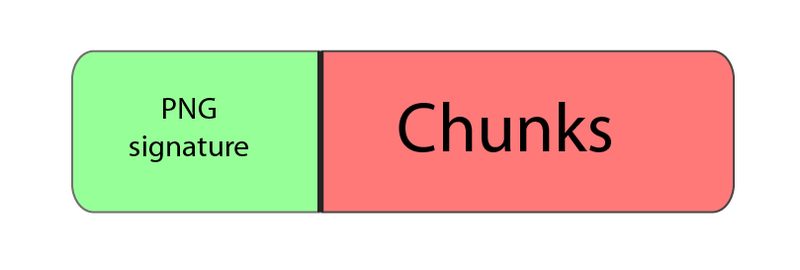
\includegraphics{PNG/1}
    \centering
    \label{img:png_1}
\end{figure}

Сигнатура PNG файла состоит из 8 байт, в hex нотации они выглядят так:
\textbf{89 50 4E 47 0D 0A 1A 0A}.

Каждый блок состоит из четырех секций: длина, тип, содержание, CRC, --- как показано на рисунке~\ref{img:png_2}:
\begin{figure}[ht!]
    \caption{Общий вид чанка}
    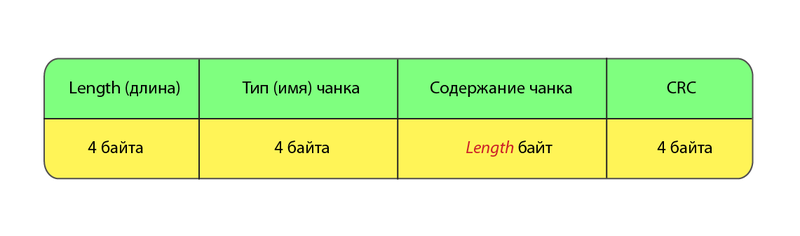
\includegraphics{PNG/2}
    \centering
    \label{img:png_2}
\end{figure}
В длине указывается длина блока в байтах. Тип указывается с помощью четырех ascii символов,
чувствительных к регистру. С помощью регистра декодеру передается дополнительная информация, а именно:
\begin{enumerate}
    \item Регистр первого символа сообщает, является данный блок критическим или нет. Критические
    блоки распознаются каждым декодером. Если декодер не может распознать тип такого блока,
    он аварийно завершает работу.
    \item Регистр второго символа задает публичность или приватность блока.
    Публичные блоки обычно официальные и хорошо задокументированы. Чтобы закодировать в библиотеку
    какую-то специфичную информацию, его тип можно изменить на приватный.
    \item Регистр третьего символа зарезервирован на будущее. По умолчанию там стоит символ в большом регистре.
    \item Регистр четвертого символа сообщает возможность копирования данного блока редакторами.
\end{enumerate}

Список критических блоков:
\begin{enumerate}
    \item IHDR --- заголовочный блок, содержающий основную информацию об изображении.
    \item PLTE --- палитра изображения.
    \item IDAT --- содержит непосредственно изображение.
    В любом PNG файле должно быть не менее одного такого блока.
    \item IEND --- завершающий чанк. Должен находиться в самом конце файла.
\end{enumerate}

Список некритических блоков:
\begin{enumerate}
    \item bKGD --- блок, задающий фоновый цвет изображения.
    \item cHRM --- блок, используемый для задания цветового пространства CIE 1931.
    \item gAMA --- определяет гамму.
    \item hIST --- хранит гистограмму изображения либо общее содержания каждого цвета в рисунке.
    \item iTXt --- содержит текст в UTF-8
    \item pHYs --- содержит размер пикселя или отношение сторон изображения.
    \item sRGB --- свидетельствует об использовании sRGM схемы.
    \item tIME --- дата последнего изменения изображения.
    \item tRNS --- информация о прозрачности.
\end{enumerate}

Согласно вышесказанному, минимальный PNG файл выглядит так,
как показано на рисунке~\ref{img:png_3}

\begin{figure}[ht!]
    \caption{Минимальный PNG}
    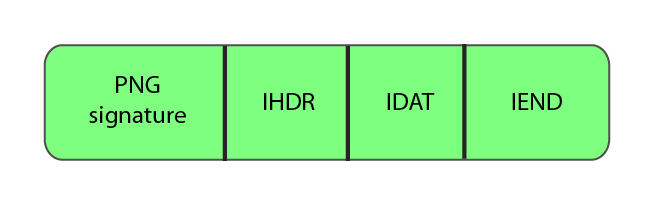
\includegraphics{PNG/3}
    \centering
    \label{img:png_3}
\end{figure}

В следующей секции представлены данные блока.
В секции CRC записан CRC блока.

Наиболее интересными для нас являются блоки с типами IHDR и IDAT.
IHDR --- заголовочный блок, который является обязательным для PNG файла.
Он содержит следующие интересующие нас поля:
\begin{enumerate}
    \item Ширина изображения в пикселях.
    \item Высота изображения в пикселях.
    \item Битовая глубина, задающее количество бит на каждый сэмпл.
    \item Тип цвета. Возможны следующие значения:
    \begin{enumerate}
        \item Градация серого
        \item RGB
        \item Индексы из палитры
        \item Градация серого и альфа-канал
        \item RGB и альфа-канал
    \end{enumerate}
\end{enumerate}

Блок IDAT содержит сжатые данные изображения.
На данный момент поддерживается только сжатие по алгоритму deflate.

\section{Реализация LSB для контейнера PNG}
PNG изображение представимо в виде матрицы, элементами которой являются пиксели.
В случае RGB каждый пиксель представляет элементы из трех каналов, каждый из каналов
в отдельности может рассматриваться как градация серого. В случае градации серого каждый
пиксель просто представлен значением от 0 до 255.
Чтобы закодировать сообщение в эту матрицу, склеим ее строки друг с другом в одну большую строку,
равно как и склеим каналы, чтобы они образовали последовательность элементов.
Именно это делает метод \textbf{\_ to \_ elements}.
Такой метод одинаково хорошо подходит и для разных типов цвета: RGB, RGB и альфа-канала,
градации серого, градации серого и альфа-канала.
Чтобы из элементов получить двумерную RGB матрицу,
проделаем обратную операцию, что и далет метод \textbf{\_ from \_ elements}.

В функции \textbf{main} используем как сообщение книгу ``Алиса в стране чудес'' в оригинале.
Считаем файл с книгой как последовательность байт и закодируем в изображение с помощью LSB.
Далее выполним декодирование и сверим полученные данные.
Исходный код представлен в листинге~\ref{code:png}.
\lstinputlisting[language=Python, label={code:png}, style=simplecode, caption=реализация LSB для PNG, frame=single]{Code/png.py}
Сравнение изображение до и после заполнения контейнера методом LSB
привидено на рисунке~\ref{img:lsb}.
Как видно, два рисунка визуально неотличимы,
хотя в одном из них закодировано 150 килобайт информации.
\begin{figure}[ht!]
    \centering
    \begin{subfigure}{.5\textwidth}
      \centering
      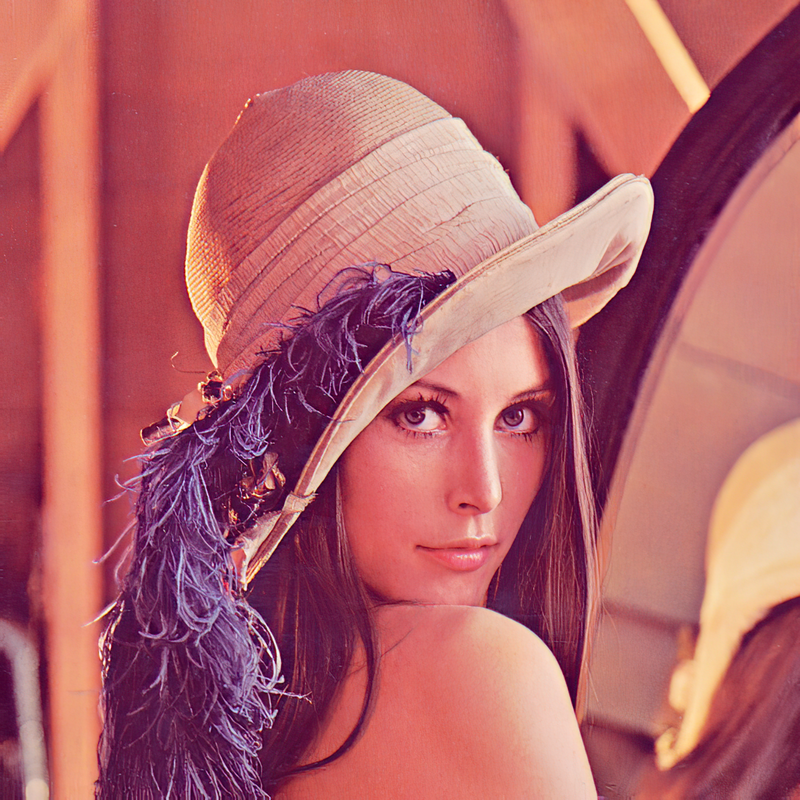
\includegraphics[width=.9\linewidth]{PNG/Lenna.png}
      \caption{Оригинал}
      \label{img:lenna-png}
    \end{subfigure}%
    \begin{subfigure}{.5\textwidth}
      \centering
      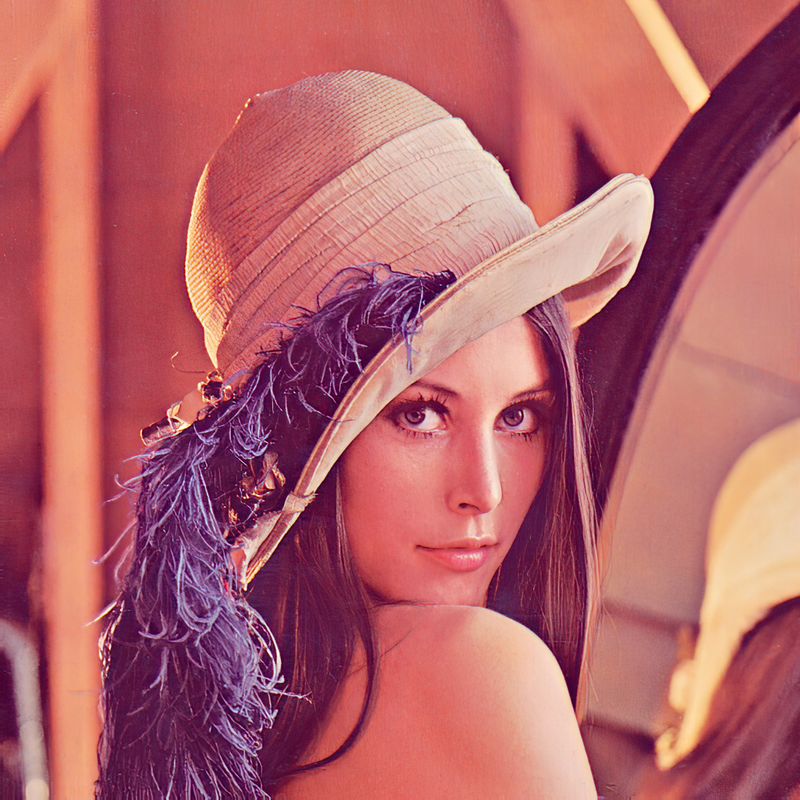
\includegraphics[width=.9\linewidth]{PNG/LSB_Lenna.png}
      \caption{После приминения LSB}
      \label{img:lenna-lsb}
    \end{subfigure}
    \caption{Изображение до и после приминения LSB}
    \label{img:lsb}
\end{figure}